\documentclass{beamer}

\usepackage[utf8]{inputenc}
\usepackage{graphicx}
\graphicspath{ {./Figures/} }

\title{Modeling Price and Popularity of AirBnB listings in New-York}
\author{Melody Jiang, Raphael Morsomme, Ezinne Nwankwo}
\institute{Department of Statistical Science, Duke University}
\date{02/03/2020}

\begin{document}

\frame{\titlepage}



%%%%%%%%%% Section1: Introduction %%%%%%%%%%%




\begin{frame}
    \frametitle{EDA - A city of two tales}

    
    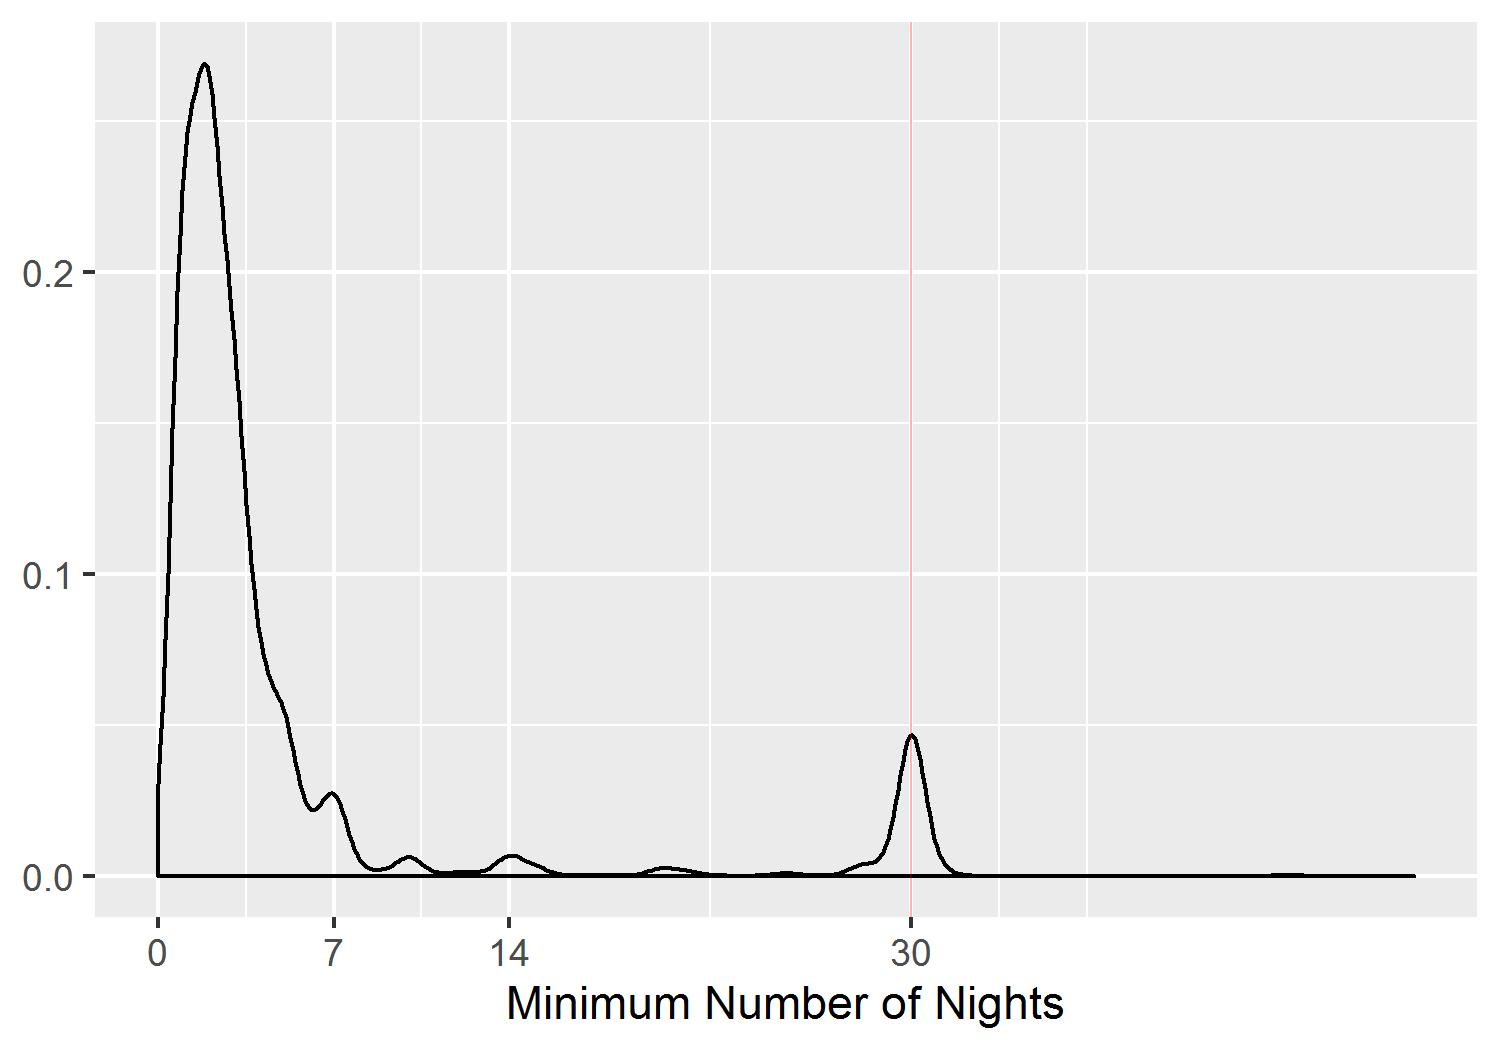
\includegraphics[scale = 0.2]{length_stay_density.jpeg}
\end{frame}


\begin{frame}
    \frametitle{EDA - Are you available?}
    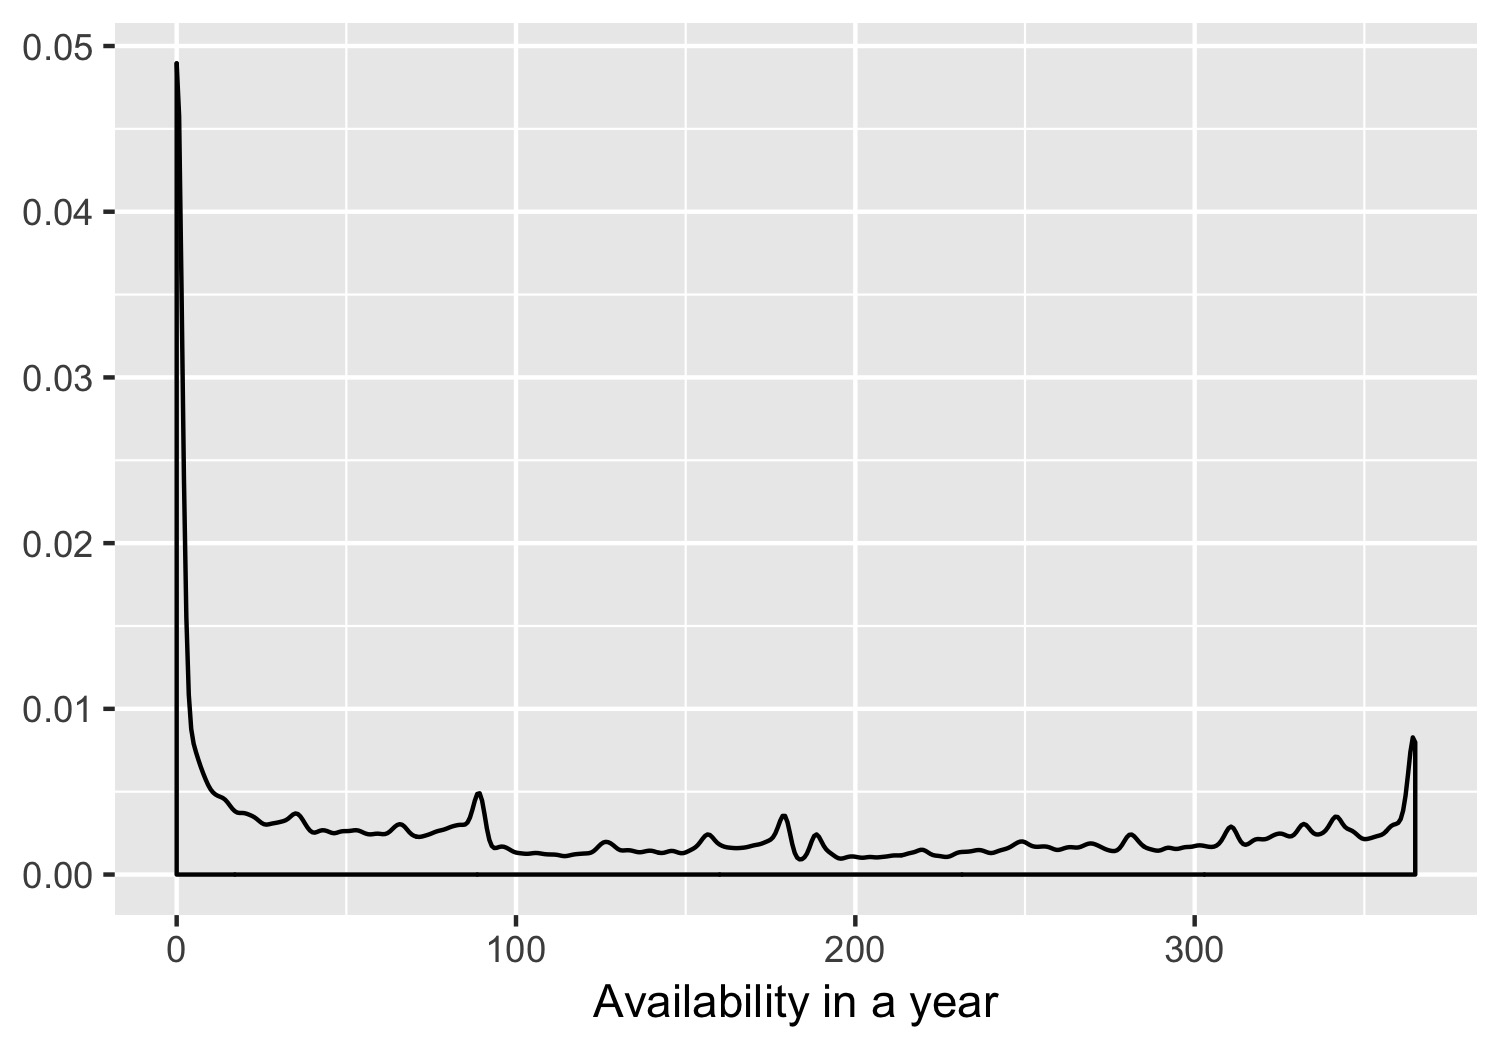
\includegraphics[scale = 0.2]{availability_density.jpeg}
\end{frame}

\begin{frame}
    \frametitle{EDA - Room type}
    \begin{itemize}
        \item $p < 1e-16$
    \end{itemize}
    \centering
    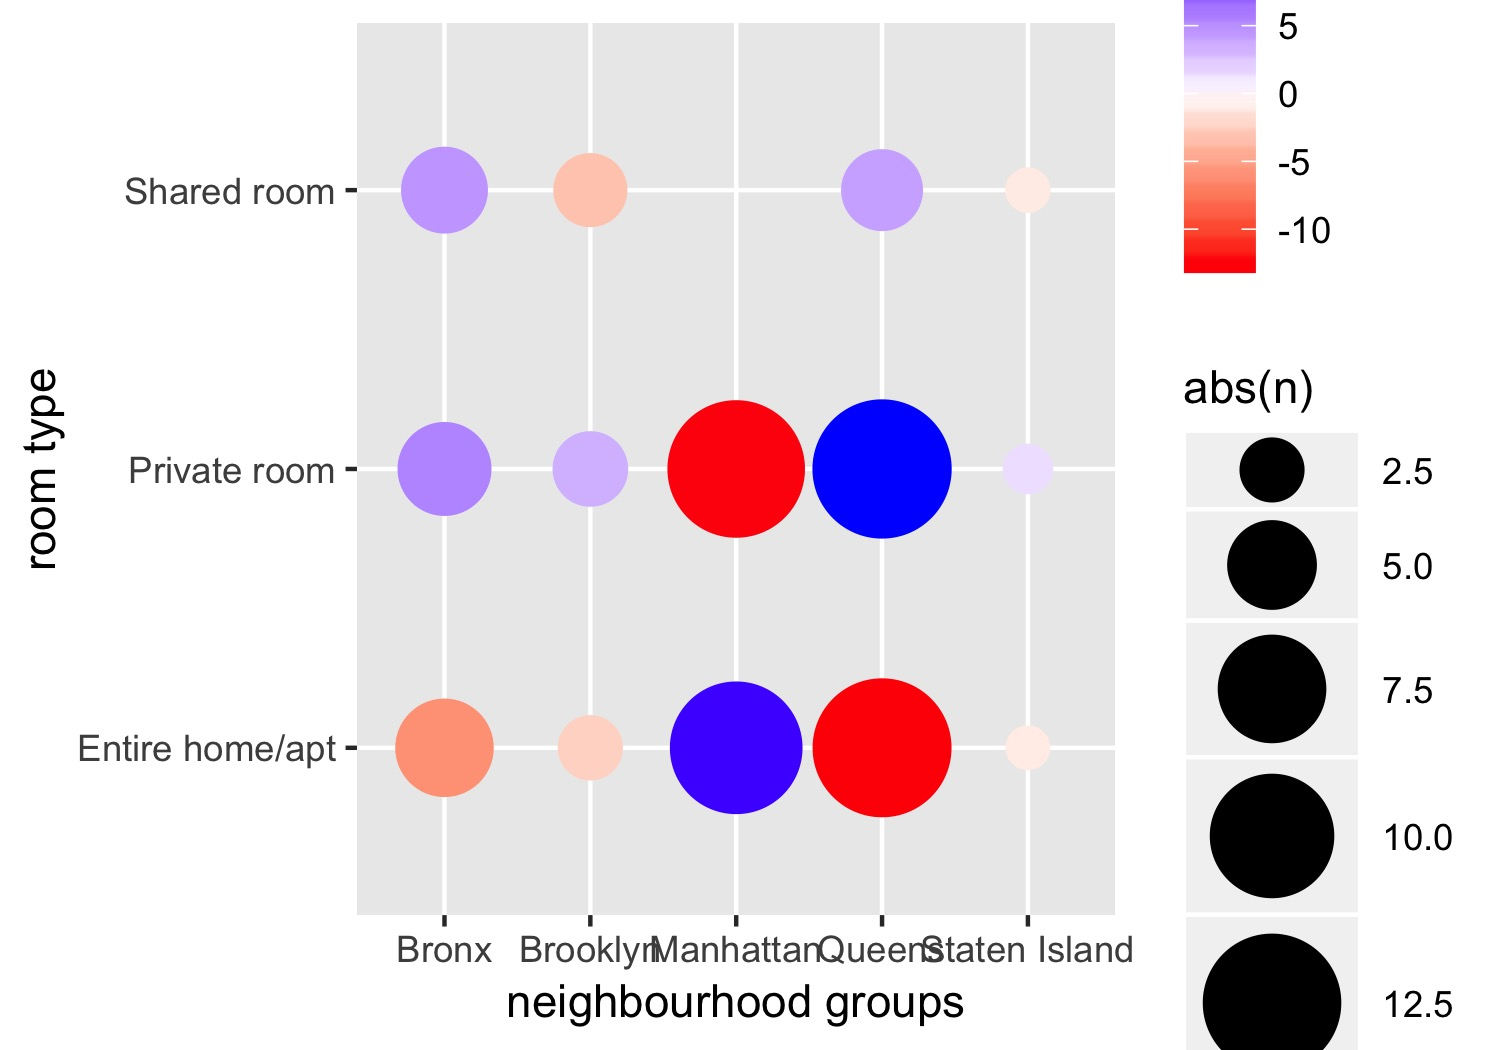
\includegraphics[scale = 0.13]{room_type_chi.jpeg}

\end{frame}

\begin{frame}
    \frametitle{EDA - Attractions}
    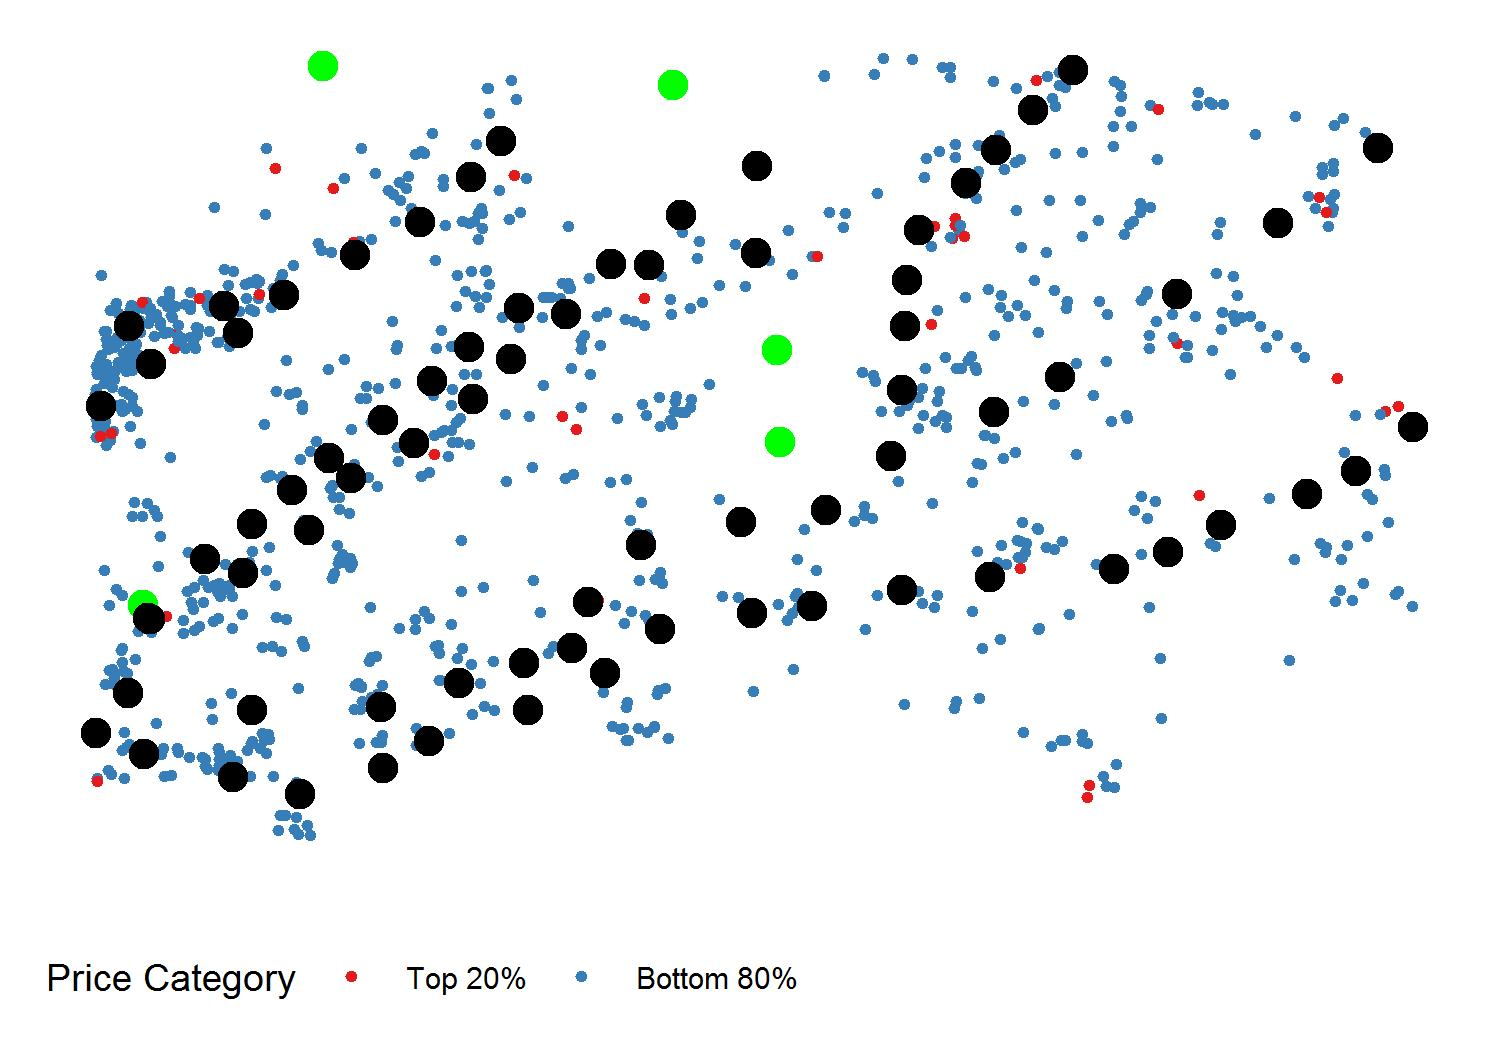
\includegraphics[scale = 0.8]{map_eda.jpeg}
\end{frame}


\begin{frame}
\frametitle{Data Cleaning}
Since the data quality is questionable, we narrow down our focus to \textit{active} listing for \textit{short term} stays that are \textit{private}:

\begin{itemize}
	\item last review is less than $12$ months old
	\item min number of days inferior to to $29$
	\item less than $5$ listings per owner
\end{itemize}

We also incorporate external data:
\begin{itemize}
	\item Location of metro stations
	\item Location of main attractions
\end{itemize}
\end{frame}



\begin{frame}
\frametitle{Feature Engineering - Proximity to Metro and Attractions}
EDA suggests spatial modeling:
\begin{itemize}
	\item Proximity to closest metro stations
	$$dist_{Manhattan}(x, y) = |lat_{x} - lat_{y}| +  |long_{x} - long_{y}|$$
	\item Average proximity to ($36$) attractions
	$$proximity(X) = \dfrac{1}{n}\sum_{i=1}^{n} \dfrac{1}{dist(X, attraction_i)}
	$$
\end{itemize}
\end{frame}



\begin{frame}
\frametitle{Feature Engineering - Textual Data}
Textual data always invites creativity:
\begin{itemize}
	\item Sentiment analysis of listing name
	$$ Sentiment(W) = \dfrac{1}{n}\sum_{i=1}^{n} dictionary(w_i)$$
	where $dictionary_{Affin}(w) \in \left\lbrace -5, -4, \dots, 5\right\rbrace$
	\item Origin of host $\Rightarrow$ frequency of name
\end{itemize}
\end{frame}

\begin{frame}
    \frametitle{Feature Engineering - Attractions}
    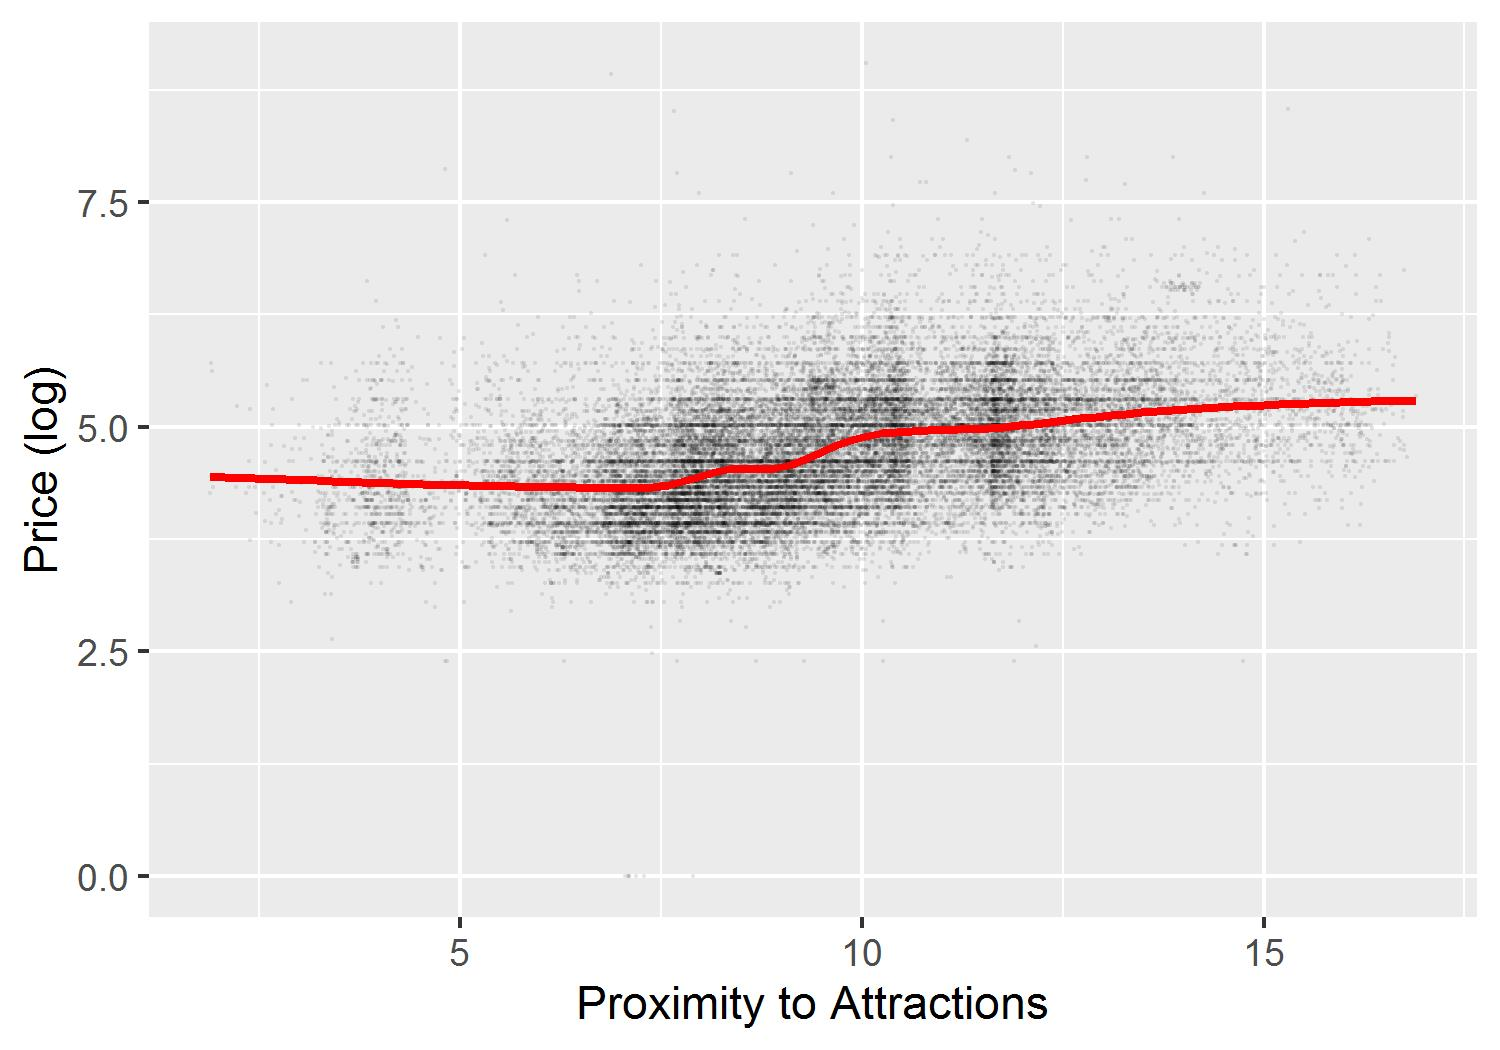
\includegraphics[scale = 0.8]{log_price_vs_prox_attr.jpeg}
\end{frame}

\begin{frame}
    \frametitle{Feature Engineering - Metro}
    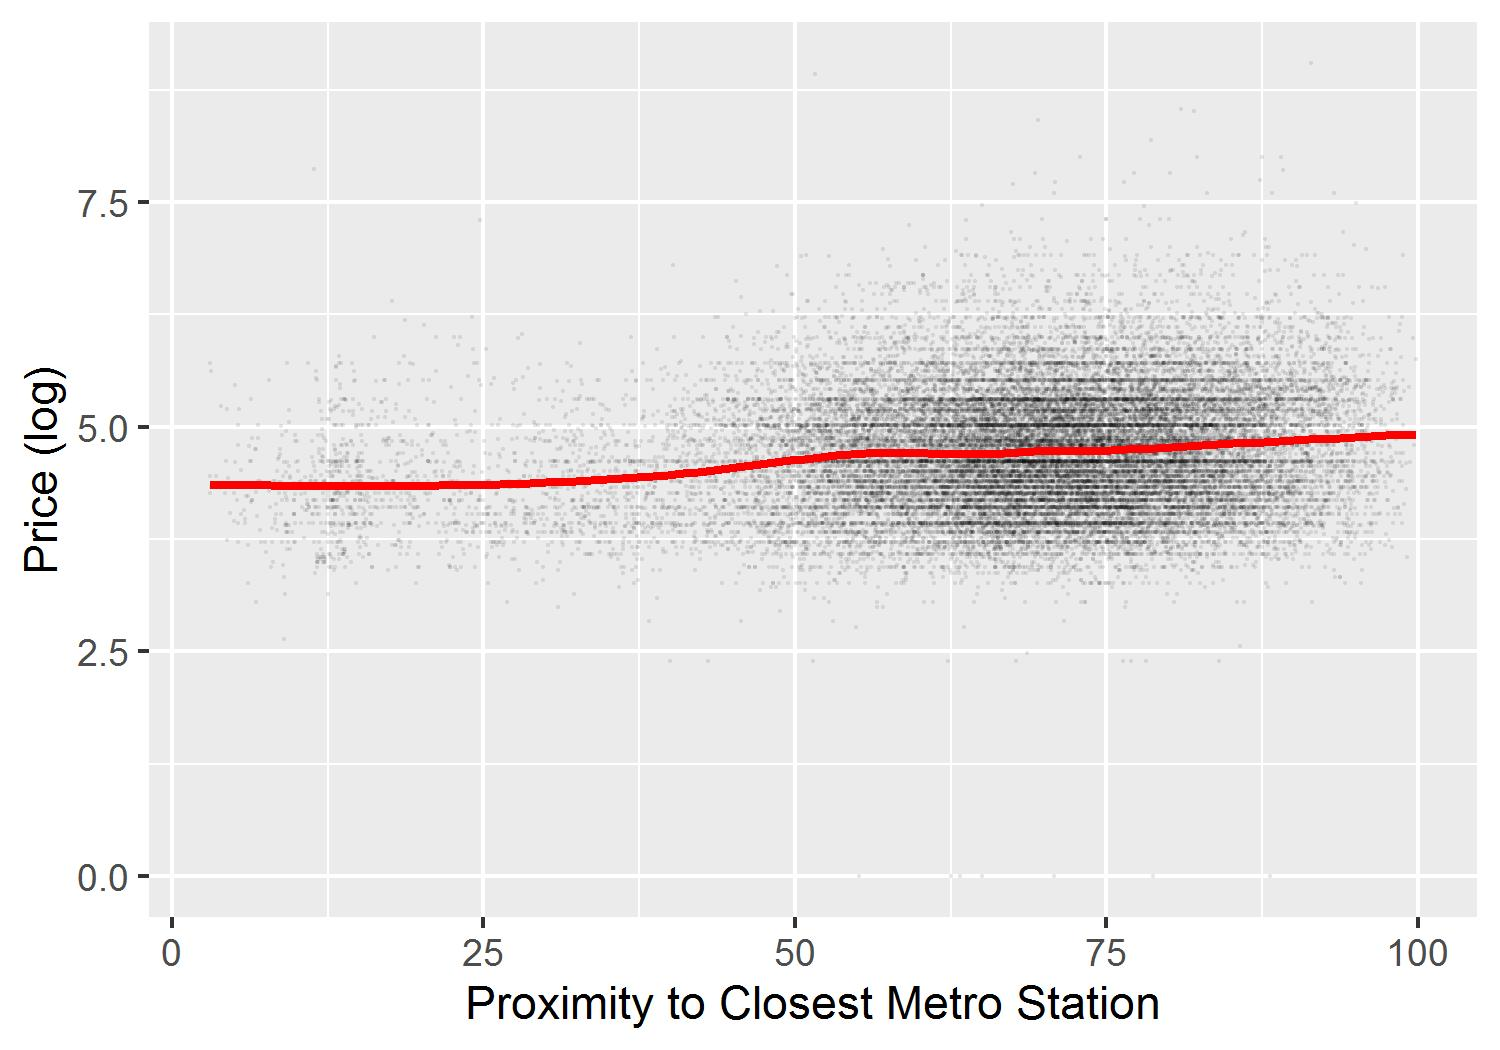
\includegraphics[scale = 0.8]{log_price_vs_prox_metro.jpeg}
\end{frame}

\begin{frame}
\frametitle{Models}
Two regression models
\begin{itemize}
	\item Regression Model
	\begin{itemize}
		\item Outcome: price, popularity
		\begin{itemize}
            \item $\text{popularity} = \frac{\text{reviews per month}}{\text{availability}}$
        \end{itemize}
		\item Predictors: listing sentiment, name frequency, proximity metro, proximity attraction, room type, etc.
		\item $n = 25,000$, $p=14$
	\end{itemize}
	\item Random Forest
	\begin{itemize}
		\item $1,900$ trees, subsamples $19,000$
		\item $m=\frac{p}{3}=4$ variables at each split, $n_{leaf} \ge 5$.
	\end{itemize}
	\item BMA
	\begin{itemize}
		\item Linear combination of predictors
		\item Prior: Cauchy
		\item N.Models: $2^{15}$
		\item MCMC.iterations: $10^{16}$
		\item initprobs $=$ "marg-eplogp"
	\end{itemize}
\end{itemize}
\end{frame}



\begin{frame}
\frametitle{Models - continued}
\begin{itemize}
	\item Important Predictors
	\begin{itemize}
		\item RF: variable importance
		
		\item BMA: PIP
	\end{itemize}
	\item Sensitivity Analysis
	\begin{itemize}
		\item RF: vary $m$ and minimum $n_{leaf}$.
		\item BMA: consider different priors (Cauchy prior, g prior for $g = 1,5,8,100,500,1000$)
	\end{itemize}
\end{itemize}

\end{frame}


%%%%%%%
\begin{frame}
\frametitle{Results - Random Forest Price}
% latex table generated in R 3.6.1 by xtable 1.8-4 package
% Mon Feb  3 21:05:30 2020
\begin{table}[ht]
\centering
\begin{tabular}{rlr}
  \hline
 & Predictors & Variable.Importance \\ 
  \hline
1 & last\_review & 978.10 \\ 
  2 & name\_listing\_sentiment & 107.88 \\ 
  3 & name\_host\_freq & 101.15 \\ 
  4 & availability\_365 & 100.73 \\ 
  5 & Room\_type & 95.16 \\ 
  6 & number of reviews & 94.24 \\ 
  7 & reviews\_per\_month & 90.71 \\ 
  8 & proximity\_metro & 89.26 \\ 
  9 & calculated\_host\_listings\_count & 88.53 \\ 
  10 & Neighbourhood\_group & 61.00 \\ 
  11 & type\_stay & 53.69 \\ 
  12 & name\_host\_special & 47.78 \\ 
  13 & name\_listing\_length & 39.16 \\ 
  14 & proximity\_attraction & 16.42 \\ 
   \hline
\end{tabular}
\end{table}

\end{frame}

\begin{frame}
\frametitle{Results - Random Forest Popularity}
% latex table generated in R 3.6.1 by xtable 1.8-4 package
% Mon Feb  3 21:49:38 2020
\begin{table}[ht]
\centering
\begin{tabular}{rlr}
  \hline
 & Predictors & Variable.Importance \\ 
  \hline
1 & number\_of\_reviews & 199.74 \\ 
  2 & latitude & 62.77 \\ 
  3 & listing\_sentiment & 59.50 \\ 
  4 & minimum\_nights & 57.85 \\ 
  5 & neighbourhood\_group & 54.93 \\ 
  6 & room\_type & 50.03 \\ 
  7 & reviews\_per\_month & 49.69 \\ 
  8 & longitude & 45.87 \\ 
  9 & name\_listing\_length & 41.50 \\ 
  10 & name\_host\_special & 35.34 \\ 
  11 & popularity\_log & 33.77 \\ 
  12 & proximity\_attraction & 20.73 \\ 
  13 & listing\_count & 8.76 \\ 
  14 & name\_host\_freq & 8.72 \\ 
  15 & proximity\_metro & 0.42 \\ 
   \hline
\end{tabular}
\end{table}

\end{frame}

\begin{frame}
\frametitle{Results - BMA Price}

% latex table generated in R 3.6.1 by xtable 1.8-4 package
% Mon Feb  3 21:53:08 2020
\begin{table}[ht]
\centering
\begin{tabular}{rlrrrl}
  \hline
 & Predictors & Estimate & Lower.Confint & Upper.Confint & Signifance \\ 
  \hline
1 & Intercept & 4.70 & 4.70 & 4.71 & * \\ 
  2 & Neighbourhood\_group:Manhattan & 0.17 & 0.15 & 0.18 & * \\ 
  3 & Neighbourhood\_group:Queens & -0.11 & -0.13 & -0.10 & * \\ 
  4 & Neighbourhood\_group:Staten Island & -0.00 & 0.00 & 0.00 &  \\ 
  5 & Neighbourhood\_group:Bronx & -0.17 & -0.20 & -0.14 & * \\ 
  6 & Room\_type:Entire home/apt & 0.74 & 0.73 & 0.75 & * \\ 
  7 & Room\_type:Shared room & -0.51 & -0.54 & -0.47 & * \\ 
  8 & number of reviews & -0.01 & -0.02 & -0.01 & * \\ 
  9 & last\_review & -0.00 & -0.00 & -0.00 & * \\ 
  10 & reviews\_per\_month & -0.00 & -0.00 & 0.00 &  \\ 
  11 & calculated\_host\_listings\_count & -0.01 & -0.02 & -0.01 & * \\ 
  12 & availability\_365 & 0.00 & 0.00 & 0.00 & * \\ 
  13 & name\_listing\_sentiment & 0.00 & 0.00 & 0.00 & * \\ 
  14 & proximity\_attraction & -0.01 & -0.04 & 0.00 &  \\ 
  15 & name\_host\_freq & 0.07 & 0.07 & 0.07 & * \\ 
  16 & name\_host\_special:True & 10.42 & 7.29 & 13.45 & * \\ 
  17 & name\_listing\_length & 0.06 & 0.04 & 0.08 & * \\ 
  18 & type\_stay:Long & 0.00 & 0.00 & 0.00 & * \\ 
  19 & proximity\_metro & -0.00 & -0.00 & 0.00 &  \\ 
   \hline
\end{tabular}
\end{table}

\end{frame}

\begin{frame}
\frametitle{Results - BMA Popularity}
\begin{center}
	% latex table generated in R 3.6.1 by xtable 1.8-4 package
% Mon Feb  3 21:53:10 2020
\begin{table}[ht]
\centering
\begin{tabular}{rlrrrl}
  \hline
 & Predictors & Estimate & Lower.Confint & Upper.Confint & Signifance \\ 
  \hline
1 & Intercept & 4.70 & 4.70 & 4.71 & * \\ 
  2 & Neighbourhood\_group:Manhattan & 0.17 & 0.15 & 0.18 & * \\ 
  3 & Neighbourhood\_group:Queens & -0.11 & -0.13 & -0.10 & * \\ 
  4 & Neighbourhood\_group:Staten Island & -0.00 & 0.00 & 0.00 &  \\ 
  5 & Neighbourhood\_group:Bronx & -0.17 & -0.20 & -0.14 & * \\ 
  6 & Room\_type:Entire home/apt & 0.74 & 0.73 & 0.75 & * \\ 
  7 & Room\_type:Shared room & -0.51 & -0.54 & -0.47 & * \\ 
  8 & number of reviews & -0.01 & -0.02 & -0.01 & * \\ 
  9 & last\_review & -0.00 & -0.00 & -0.00 & * \\ 
  10 & reviews\_per\_month & -0.00 & -0.00 & 0.00 &  \\ 
  11 & calculated\_host\_listings\_count & -0.01 & -0.02 & -0.01 & * \\ 
  12 & availability\_365 & 0.00 & 0.00 & 0.00 & * \\ 
  13 & name\_listing\_sentiment & 0.00 & 0.00 & 0.00 & * \\ 
  14 & proximity\_attraction & -0.01 & -0.04 & 0.00 &  \\ 
  15 & name\_host\_freq & 0.07 & 0.07 & 0.07 & * \\ 
  16 & name\_host\_special:True & 10.42 & 7.29 & 13.45 & * \\ 
  17 & name\_listing\_length & 0.06 & 0.04 & 0.08 & * \\ 
  18 & type\_stay:Long & 0.00 & 0.00 & 0.00 & * \\ 
  19 & proximity\_metro & -0.00 & -0.00 & 0.00 &  \\ 
   \hline
\end{tabular}
\end{table}

\end{center}

\end{frame}


\begin{frame}
\frametitle{Diagnostic Plots - BMA - Popularity}
\begin{center}
	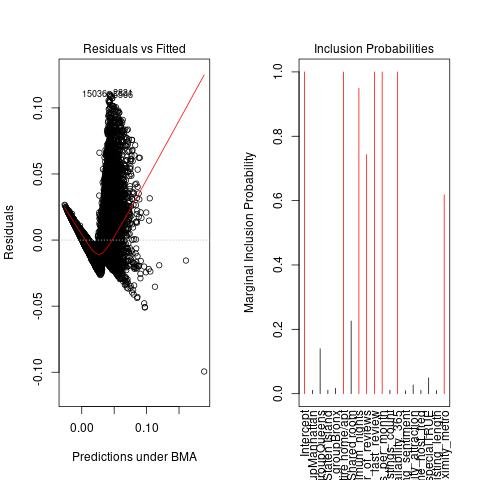
\includegraphics[scale = 0.5]{diagnostics_pop_bma.jpeg}	
\end{center}
\end{frame}



\begin{frame}
\frametitle{Residuals - BMA}
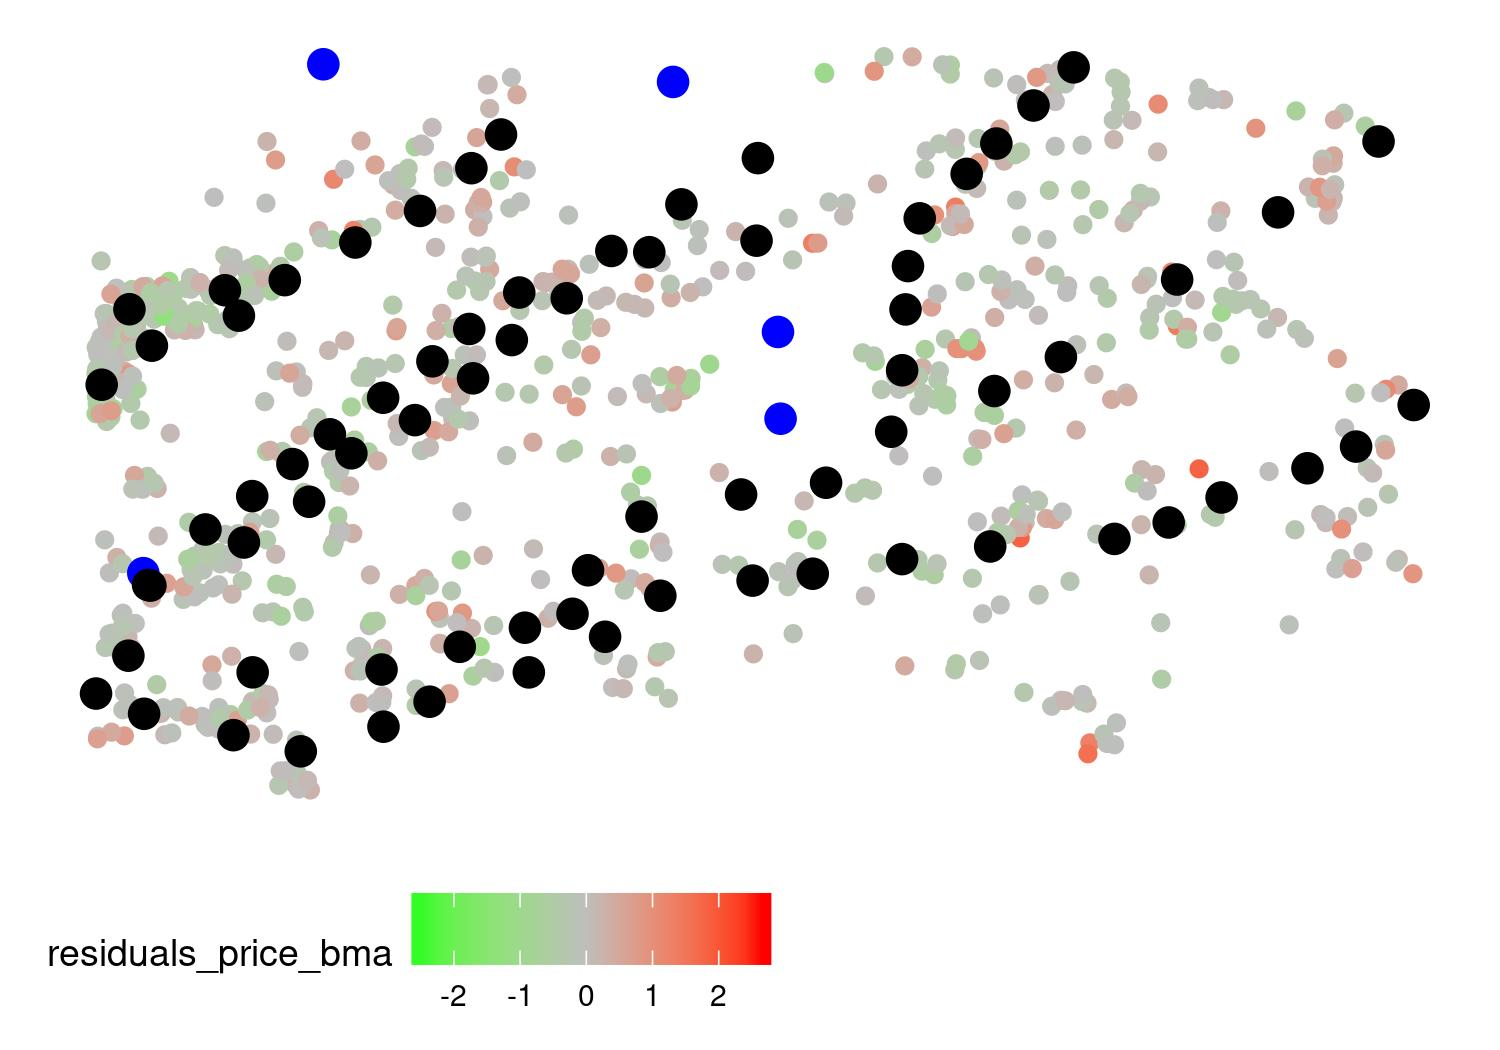
\includegraphics[scale = 0.9]{map_price_bma.jpeg}
\end{frame} 

%%%%%%%


\begin{frame}
    \frametitle{Discussions - Future Directions}

    \begin{itemize}
        \item Data collection
        \begin{itemize}
            \item One row per booking
        \end{itemize}
        \item Spatial modeling
        \begin{itemize}
            \item Incusion of boroughs does not work well. Spatial modeling that addresses relationship between houses (Valente, 2005).
        \end{itemize}
        \item Domain-specific knowledge
        \begin{itemize}
            \item Submarkets influence pricing. Finite mixture model by Belasco1, 2012.
            \item Knowledge in marketing. E.g. consider form of pricing as an influencer of popularity (99 vs 100).
        \end{itemize}
    \end{itemize}

\end{frame}


\begin{frame}
    \frametitle{Discussions}

    \centering
    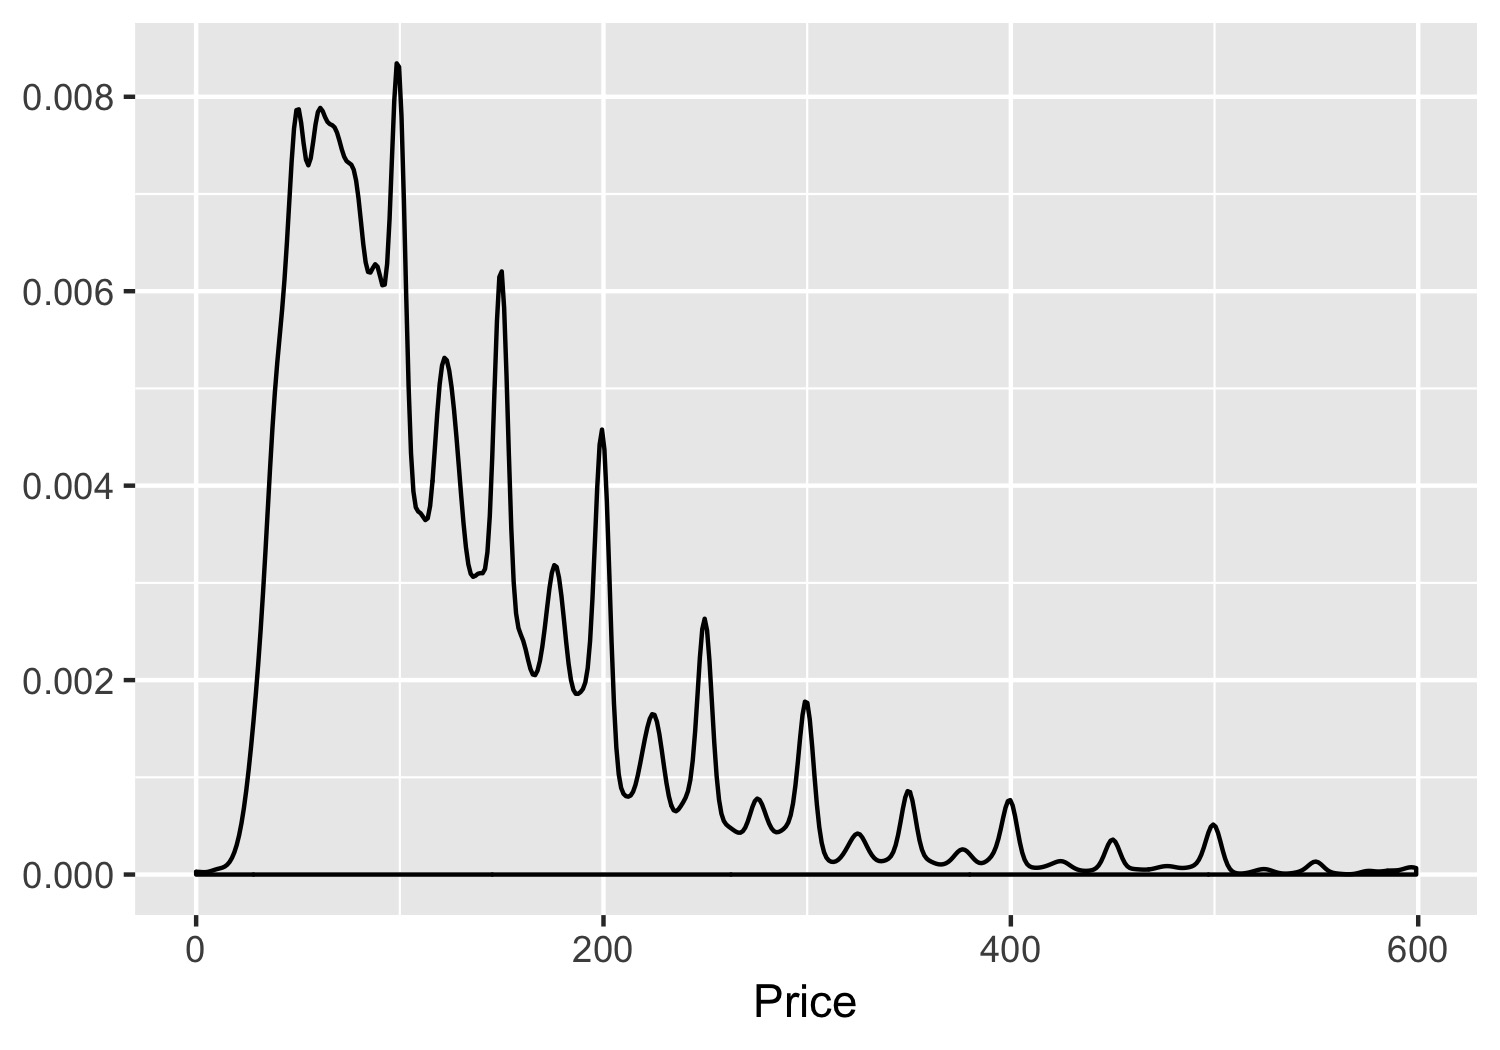
\includegraphics[scale = 0.2]{price.jpeg}
\end{frame}



\begin{frame}
\frametitle{References}
\footnotesize{
	\begin{thebibliography}{99} % Beamer does not support BibTeX so references must be inserted manually as below
		
		\bibitem[Whickam, 2013]{Whickam2009} Whickam, H. \\
		\newblock Tidy Data\\
		\newblock \emph{Journal}, month year
		
    \end{thebibliography}
    
    \begin{thebibliography}{99} % Beamer does not support BibTeX so references must be inserted manually as below
		
		\bibitem[Valente, 2005]{Valente2005} Valente, j. \\
		\newblock Apartment Rent Prediction Using Spatial Modeling\\
		\newblock \emph{Journal}, month year
		
    \end{thebibliography}
    
    \begin{thebibliography}{99} % Beamer does not support BibTeX so references must be inserted manually as below
		
		\bibitem[Belasco, 2012]{Belasco2012} Belasco, E. \\
		\newblock Using a Finite Mixture Model of Heterogeneous Households to Delineate Housing Submarkets\\
		\newblock \emph{Journal}, month year
		
	\end{thebibliography}
}
\end{frame}
    






\end{document}
